\documentclass[10pt,twocolumn,letterpaper]{article}

%% paquetes esenciales
\usepackage[utf8]{inputenc}
\usepackage[T1]{fontenc}
\usepackage[spanish]{babel}
\usepackage{amsmath,amssymb}
\usepackage{graphicx}
\usepackage{subcaption}
\usepackage{booktabs}
\usepackage{multirow}
\usepackage[colorlinks=true,linkcolor=blue!70!black,
            citecolor=blue!70!black,urlcolor=blue!70!black]{hyperref}
\usepackage{xcolor}
\usepackage{geometry}
\usepackage{natbib}
\usepackage{titlesec}
\usepackage{abstract}
\usepackage{fancyhdr}
\usepackage{parskip}
\usepackage{caption}
\usepackage{enumitem}
\usepackage{lmodern}

%% maquetado
\geometry{
  letterpaper,
  top=1.8cm, bottom=2.2cm,
  left=1.5cm, right=1.5cm,
  columnsep=0.6cm
}

%% encabezado
\pagestyle{fancy}
\fancyhf{}
\renewcommand{\headrulewidth}{0.4pt}
\fancyhead[L]{\small\textit{\moppo{}: MORL para Anonimizacion de Grafos}}
\fancyhead[R]{\small\textit{Estrada Montano \& Alanis Gonzalez, 2026}}
\fancyfoot[C]{\small\thepage}

%% secciones compactas
\titleformat{\section}{\normalfont\large\bfseries}{\thesection.}{0.5em}{}
\titleformat{\subsection}{\normalfont\normalsize\bfseries}{\thesubsection.}{0.5em}{}
\titleformat{\subsubsection}[runin]{\normalfont\normalsize\bfseries}{}{0em}{}[.]
\titlespacing{\section}{0pt}{8pt plus 2pt minus 2pt}{4pt}
\titlespacing{\subsection}{0pt}{6pt plus 2pt minus 2pt}{2pt}

%% abstract en dos columnas
\renewcommand{\abstractnamefont}{\normalfont\bfseries}
\renewcommand{\abstracttextfont}{\normalfont\small}
\setlength{\absleftindent}{0pt}
\setlength{\absrightindent}{0pt}

%% captions mas compactos
\captionsetup{font=small, labelfont=bf, skip=4pt}
\captionsetup[subfigure]{font=small, labelfont=bf}

%% parrafos
\setlength{\parskip}{3pt}
\setlength{\parindent}{1em}

%% macros
\newcommand{\moppo}{\textsc{moppo}}
\newcommand{\rpriv}{r_{\text{priv}}}
\newcommand{\rutil}{r_{\text{util}}}
\newcommand{\HV}{\text{HV}}
\newcommand{\Ddelta}{\Delta}

% ======================================================================
\begin{document}

%% bloque de titulo en una sola columna
\twocolumn[{%
\begin{@twocolumnfalse}

\vspace*{0.3cm}
{\centering
  {\LARGE\bfseries
    \moppo: Aprendizaje por Refuerzo Multi-Objetivo\\[4pt]
    con Curriculum Learning para Anonimizacion de Grafos}\\[10pt]
  {\large Analisis de equidad mediante TREX y auditoria por cuartil de grado}
  \par}

\vspace{10pt}

{\centering
\begin{tabular}{cc}
  \begin{minipage}{0.45\textwidth}\centering
    {\bfseries Abril Minerva Estrada Montano}\\[2pt]
    \small Licenciatura en Ciencia de Datos\\
    \small \texttt{abrilminerva@gmail.com}
  \end{minipage}
  &
  \begin{minipage}{0.45\textwidth}\centering
    {\bfseries Sebastian Alanis Gonzalez}\\[2pt]
    \small Licenciatura en Ciencia de Datos\\
    \small \texttt{sebastian.alanis@gmail.com}
  \end{minipage}
\end{tabular}
\par}

\vspace{8pt}
{\centering\small Junio 2026\par}

\vspace{10pt}
\noindent\rule{\linewidth}{0.8pt}
\vspace{4pt}

\begin{abstract}
Anonimizar una red social sin destruir su estructura es un problema de optimizacion
con dos objetivos que se oponen: mientras mas privado queda el grafo, mas se aleja de
su topologia original. Nosotros formulamos esto como un problema de aprendizaje por
refuerzo multi-objetivo (MORL) y entrenamos un agente PPO condicionado por pesos para
navegar ese balance de manera adaptativa. El resultado es \moppo{}, un framework que
aprende politicas para cualquier preferencia privacidad/utilidad con un solo modelo,
en lugar de entrenar uno diferente por cada punto del frente de Pareto. Introducimos
dos contribuciones tecnicas: \emph{action masking} basado en deficit de $k$-anonimato,
que reduce el espacio efectivo de acciones entre $25\times$ y $45\times$, y un
curriculum en tres fases que resuelve la inestabilidad de gradientes contrapuestos en
el entrenamiento temprano. Evaluamos sobre el grafo de karate club ($k=2$, $k=4$) y
un subgrafo de ego de Facebook con 100 nodos, alcanzando hipervolumenes de 0.973,
0.388 y 0.897 respectivamente. Ademas documentamos un sesgo de equidad sistematico:
los nodos perifericos absorben entre $2.1\times$ y $3.9\times$ mas impacto relativo
que los hubs durante la anonimizacion, independientemente del valor de~$\alpha$.
\end{abstract}

\vspace{4pt}
\noindent\textbf{Palabras clave:} anonimizacion de grafos,
aprendizaje por refuerzo multi-objetivo, PPO, curriculum learning,
$k$-anonimato, equidad algoritmica.

\vspace{4pt}
\noindent\rule{\linewidth}{0.4pt}
\vspace{8pt}

\end{@twocolumnfalse}
}]

% ======================================================================
\section{Introduccion}

La privacidad en redes sociales lleva mas de una decada siendo estudiada, pero el
problema practico sigue abierto. Los algoritmos clasicos de anonimizacion, como el
esquema de grados de \citet{liu2008towards}, estan disenados para minimizar cambios
estructurales con una funcion de costo fija, sin preguntarse que tipo de perturbaciones
son mas aceptables segun el contexto. No hay preferencia configurable, no hay balance
explicito entre objetivos.

Nosotros partimos de una premisa distinta. La decision de cuanta privacidad comprar a
que costo en utilidad es contextual: un sistema de salud necesita maxima privacidad
aunque pierda estructura de red; una plataforma de recomendaciones no puede permitirse
perder clustering. Dado que ese balance varia por caso de uso, tiene sentido aprender
a navegar todo el frente de Pareto en lugar de resolver un unico punto.

El aprendizaje por refuerzo multi-objetivo (MORL) es el marco natural para esto.
Condicionamos la politica por un vector de pesos $\alpha \in [0,1]$ que representa la
preferencia entre privacidad y utilidad; el agente aprende a adaptar su comportamiento
segun ese vector. En la practica hay dos obstaculos: el espacio de acciones en un
grafo de $n$ nodos tiene $\binom{n}{2}+1$ posibilidades (4{,}951 para $n=100$), y
aprender ambos objetivos desde cero genera gradientes contrapuestos que desestabilizan
el entrenamiento.

Las contribuciones de este trabajo son: (i) formulacion de la anonimizacion de grafos
como MDP multi-objetivo con weight conditioning; (ii) action masking por deficit de
$k$-anonimato que reduce el espacio efectivo $25$--$45\times$; (iii) curriculum en
tres fases que estabiliza el entrenamiento; (iv) auditoria de equidad sistematica con
el indice $\Ddelta$ y analisis TREX.

% ======================================================================
\section{Trabajo relacionado}

\subsubsection*{Anonimizacion de grafos}
\citet{liu2008towards} proponen modificar la secuencia de grados para lograr
$k$-anonimato con el minimo numero de cambios de aristas. \citet{zhou2008preserving}
extienden esto a vecindarios. Ambos son metodos deterministicos con un unico objetivo.
\citet{Chester2013} demuestran que el problema es NP-hard en el caso general.
\citet{Mauw2021} destacan que la mayoria de los metodos ignoran quien dentro del grafo
paga el costo de la anonimizacion, lo que nosotros medimos con $\Ddelta$.

\subsubsection*{RL para grafos}
\citet{you2018graph} y \citet{zhou2019optimization} usan RL para generacion molecular
y sintesis de redes. Para anonimizacion, \citet{Gao2022} proponen un DQN con
recompensa binaria de privacidad, sin considerar utilidad.

\subsubsection*{MORL y weight conditioning}
\citet{Abels2019} proponen weight conditioning para redes Q; \citet{Yang2019} lo
extienden con envelope MORL. \citet{Hung2022} aplican weight conditioning a PPO para
planificacion. Nosotros adaptamos este paradigma a la modificacion de grafos y
agregamos action masking y curriculum.

% ======================================================================
\section{Formulacion del problema}

Sea $G_0 = (V, E_0)$ con $n = |V|$ nodos. Un grafo $G$ es \emph{$k$-anonimo por
grado} si:
\begin{equation}
  \forall v \in V:\; \bigl|\{u : \deg_G(u) = \deg_G(v)\}\bigr| \geq k.
\end{equation}

\paragraph{Recompensas.}
\begin{equation}
  \rpriv(G) = -\tfrac{1}{n}\!\sum_{v}\max\!\bigl(0,\,k - |\text{clase}(v)|\bigr)
\end{equation}
\vspace{-8pt}
\begin{equation}
  \rutil^{\text{proxy}} = -|\text{aristas neto modificadas}|\,/\,|E_0|
\end{equation}
\vspace{-8pt}
\begin{equation}
  \rutil^{\text{real}} = -|C(G) - C(G_0)|
\end{equation}
donde $C(\cdot)$ es el coeficiente de clustering promedio. La recompensa escalar es:
\begin{equation}
  r = \alpha\cdot\rpriv + (1{-}\alpha)\cdot\rutil^{\text{proxy}},\quad \alpha\in[0,1].
\end{equation}

\paragraph{Observacion.}
$s \in \mathbb{R}^{2n+2}$: grados normalizados, deficit de anonimato por nodo, y
vector $[\alpha, 1{-}\alpha]$.

\paragraph{Acciones.}
$\mathcal{A} = \{\text{flip}(u,v): u\!<\!v\}\cup\{\text{no-op}\}$,
$|\mathcal{A}| = \binom{n}{2}+1$.

% ======================================================================
\section{Metodologia}

\subsection{Arquitectura del modelo}

Red actor-critico con dos capas lineales de $d_h$ unidades (tanh), cabeza de actor
sobre $|\mathcal{A}|$ acciones y cabeza critica escalar. Inicializacion ortogonal:
ganancia 0.01 para el actor, 1.0 para el critico. El vector $\alpha$ entra concatenado
al estado en cada paso.

\subsection{Enmascaramiento de acciones}

Calculamos los nodos en riesgo:
$\mathcal{R}_t = \{v : |\text{clase}(v)| < k\}$.
Solo son validas las aristas incidentes en $\mathcal{R}_t$ y la accion no-op:
\begin{equation}
  \mathcal{A}_t^{\text{valid}} =
    \{\text{flip}(u,v): u{\in}\mathcal{R}_t \text{ o } v{\in}\mathcal{R}_t\}
    \cup \{\text{no-op}\}.
\end{equation}

Las acciones invalidas reciben logit $-10^9$. La mascara se almacena en el buffer de
rollout y se reaplicar durante el update de PPO --- paso critico: si se omite, los
ratios $\exp(\log\pi_\theta - \log\pi_{\theta_\text{old}})$ son incorrectos y el
entrenamiento diverge.

\subsection{Curriculum Learning}

\begin{table}[h]
\centering\small
\caption{Fases del curriculum.}
\label{tab:curriculum}
\begin{tabular}{lll}
\toprule
Fase & Iters & Distribucion de $\alpha$ \\
\midrule
1 — Privacidad & $[0, T_1)$   & $\mathcal{U}(0.95, 1.0)$ \\
2 — Utilidad   & $[T_1, T_2)$ & $\mathcal{U}(0.00, 0.05)$ \\
3 — Mixto      & $[T_2, T)$   & $\mathcal{U}(0, 1)$ \\
\bottomrule
\end{tabular}
\end{table}

En la Fase 1 el agente aprende que aristas flipear para mejorar $k$-anonimato. En la
Fase 2 aprende que con $\alpha\approx 0$ la politica optima es mayoritariamente no-op.
En la Fase 3 interpola entre los comportamientos ya aprendidos, eliminando la
ambiguedad de gradientes contrapuestos.

\subsection{Actualizacion PPO}

PPO con clipping ($\varepsilon=0.2$), ventaja normalizada, 4 epocas por rollout,
$\beta_{\text{ent}}=0.05$, GAE ($\gamma=0.99$, $\lambda=0.95$), 512 pasos por
iteracion, Adam ($\text{lr}=3\times10^{-4}$), clip de gradiente en 0.5.

\subsection{Analisis de equidad con TREX}

El indice de disparidad compara la perdida de aristas entre cuartiles de grado:
\begin{equation}
  \Ddelta = \frac{\text{perdida normalizada}_{Q_1}}{\text{perdida normalizada}_{Q_4}}.
\end{equation}
$\Ddelta=1$ es equitativo; $\Ddelta>1$ indica que los nodos perifericos pagan mas.

El analisis TREX \citep{Rajapakse2026} corre 30 episodios con $\alpha$ aleatorio,
registra el perfil acumulado de recompensas y aplica $k$-means ($k=3$). Si los
clusters se separan por $\alpha$, el weight conditioning funciona correctamente.

% ======================================================================
\section{Experimentos}

\subsection{Configuraciones}

Evaluamos en: karate club \citep{Zachary1977} ($n=34$, $k=2$ y $k=4$) y un subgrafo
de ego de Facebook \citep{Leskovec2012} ($n=100$, $k=2$). Hiperparametros: $T=50$
pasos/episodio, semilla 42, $d_h=128$ (karate) y $d_h=256$ (Facebook), 500 iters
(karate) y 800 iters (Facebook).

\subsection{Metrica principal: hipervolumen}

\begin{equation}
  \HV(\mathcal{F},\mathbf{r}) = \lambda\!\Bigl(\bigcup_{p\in\mathcal{F}}[p,\mathbf{r}]\Bigr),
  \quad \mathbf{r}=(-1,-1).
\end{equation}
Evaluamos 21 valores de $\alpha\in[0,1]$, 15 episodios cada uno.

\subsection{Baselines}

Tres variantes de PPO con $\alpha$ fijo y sin curriculum: $\alpha=0$ (utilidad pura),
$\alpha=0.5$ (escalarizacion fija), $\alpha=1$ (privacidad pura). Cada baseline
entrena un modelo separado y solo es competitivo en su $\alpha$ especifico.

% ======================================================================
\section{Resultados}

\subsection{Curvas de entrenamiento}

\begin{figure}[t]
  \centering
  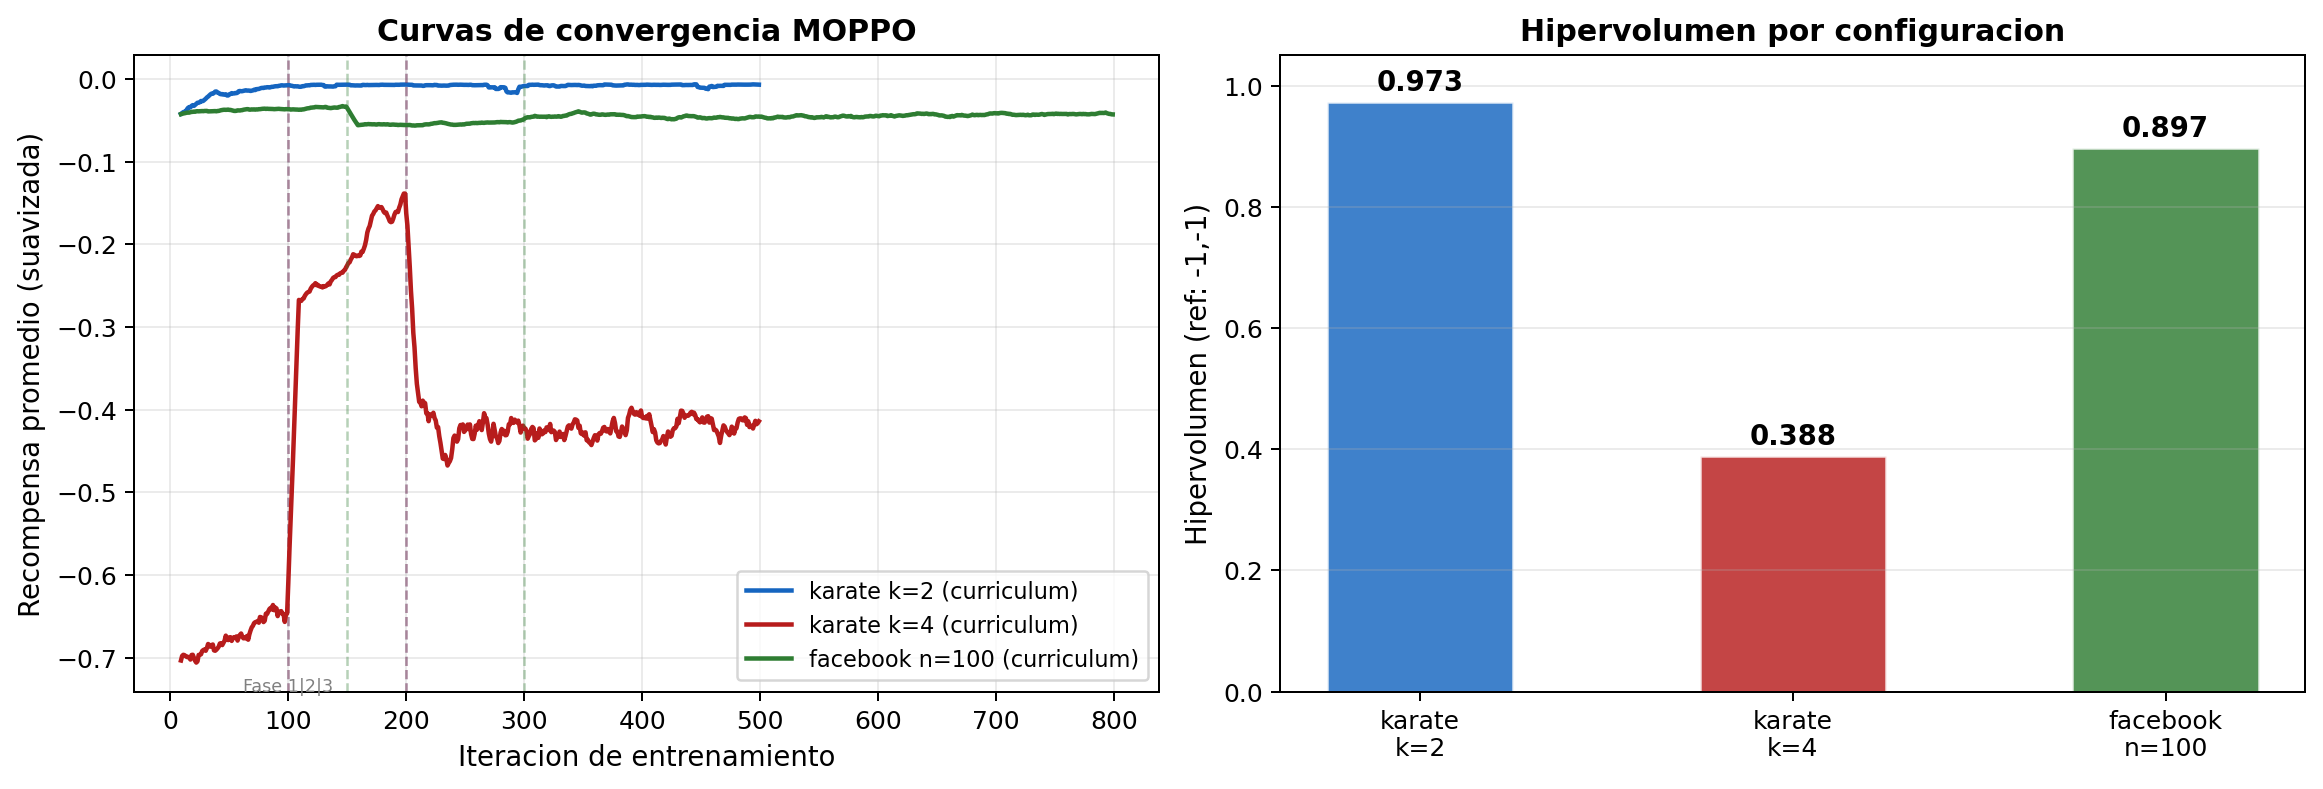
\includegraphics[width=\linewidth]{../outputs/figures/fig_training_hv.png}
  \caption{Curvas de convergencia suavizadas (ventana 10 iters). Las lineas punteadas
  verticales marcan las transiciones entre fases. El panel derecho muestra el
  hipervolumen final por configuracion.}
  \label{fig:training}
\end{figure}

La Figura~\ref{fig:training} muestra que la Fase 1 produce la mejora mas rapida en
las tres configuraciones. Para karate $k=2$ la recompensa pasa de $-0.042$ a $-0.007$
(mejora del 83.5\%). Las transiciones entre fases son suaves, sin caidas abruptas que
indicarian olvido catastrofico. La Fase 2 es la mas estable (menor desviacion estandar
en todas las configuraciones), lo que confirma que el agente ya sabe hacer no-op desde
la Fase 1.

\subsection{Frentes de Pareto}

\begin{figure*}[t]
  \centering
  \begin{subfigure}[b]{0.32\textwidth}
    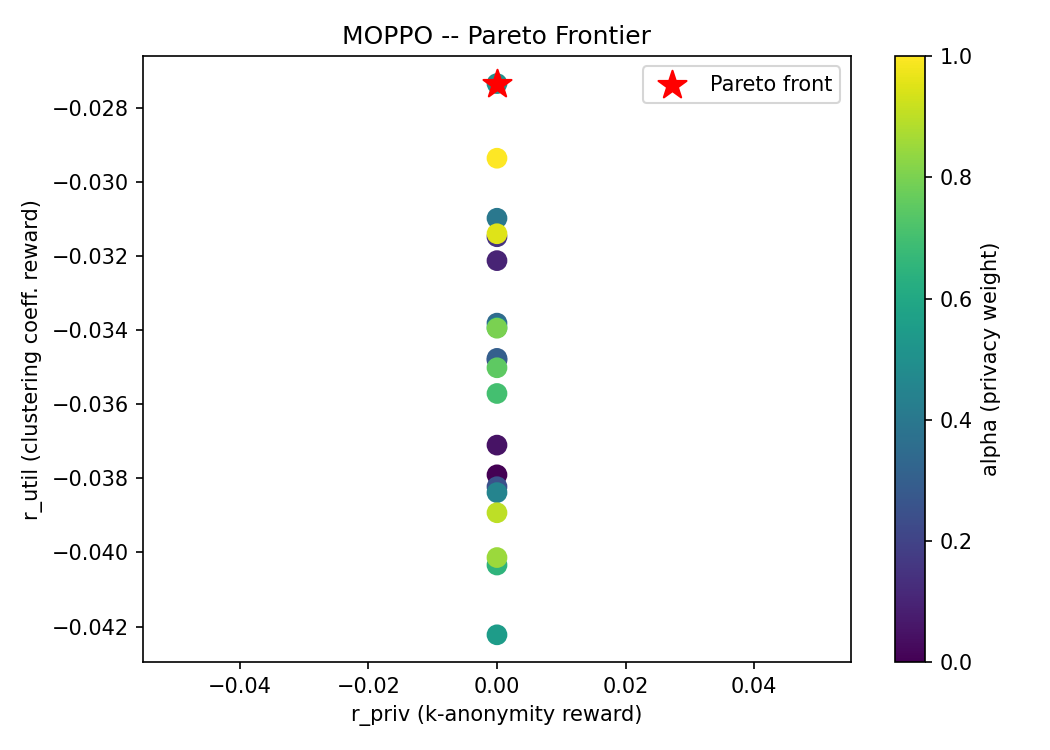
\includegraphics[width=\linewidth]{../outputs/eval_curriculum/pareto_frontier.png}
    \caption{Karate $k=2$. $\HV=0.973$, 1 pto.}
  \end{subfigure}
  \hfill
  \begin{subfigure}[b]{0.32\textwidth}
    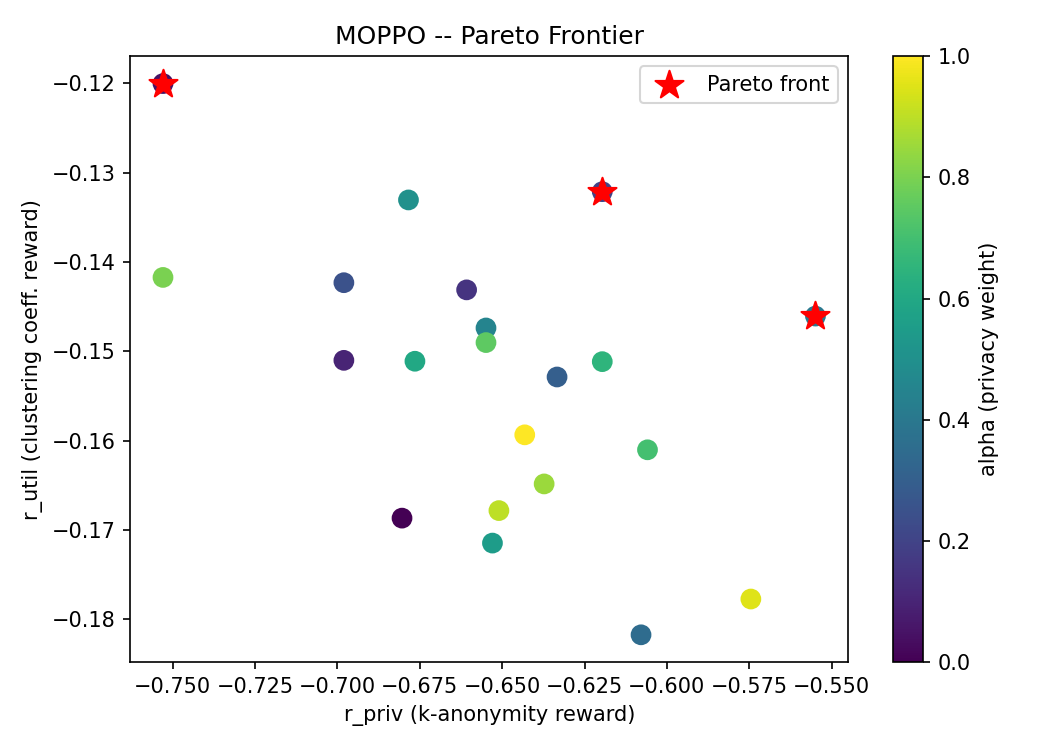
\includegraphics[width=\linewidth]{../outputs/eval_k4/pareto_frontier.png}
    \caption{Karate $k=4$. $\HV=0.388$, 3 ptos.}
  \end{subfigure}
  \hfill
  \begin{subfigure}[b]{0.32\textwidth}
    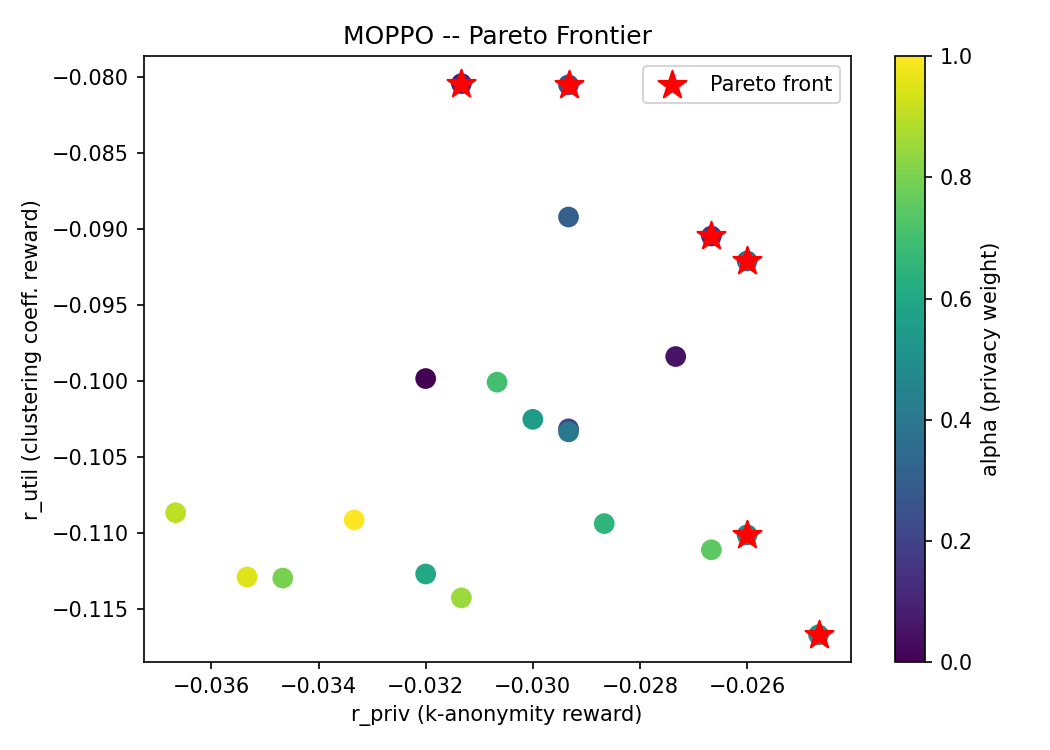
\includegraphics[width=\linewidth]{../outputs/eval_fb/pareto_frontier.png}
    \caption{Facebook $n=100$. $\HV=0.897$, 6 ptos.}
  \end{subfigure}
  \caption{Frentes de Pareto de \moppo{}. Color del punto: $\alpha$
  (azul/morado~$=$~utilidad, amarillo/verde~$=$~privacidad). Estrellas rojas: puntos
  no dominados.}
  \label{fig:pareto}
\end{figure*}

La Figura~\ref{fig:pareto} muestra los tres frentes. En karate $k=2$ el frente
degenera a un punto porque el modelo alcanza $k$-anonimato perfecto para todos los
$\alpha$; la variacion esta solo en utilidad ($\rutil\in[-0.042,-0.027]$). Karate
$k=4$ muestra el tradeoff mas claro: tres puntos con rango de 0.202 en $\rpriv$.
Facebook $n=100$ produce el frente mas rico: seis puntos con distribucion de colores
que confirma el weight conditioning.

\subsection{Analisis TREX}

\begin{figure}[t]
  \centering
  \begin{subfigure}[b]{0.48\columnwidth}
    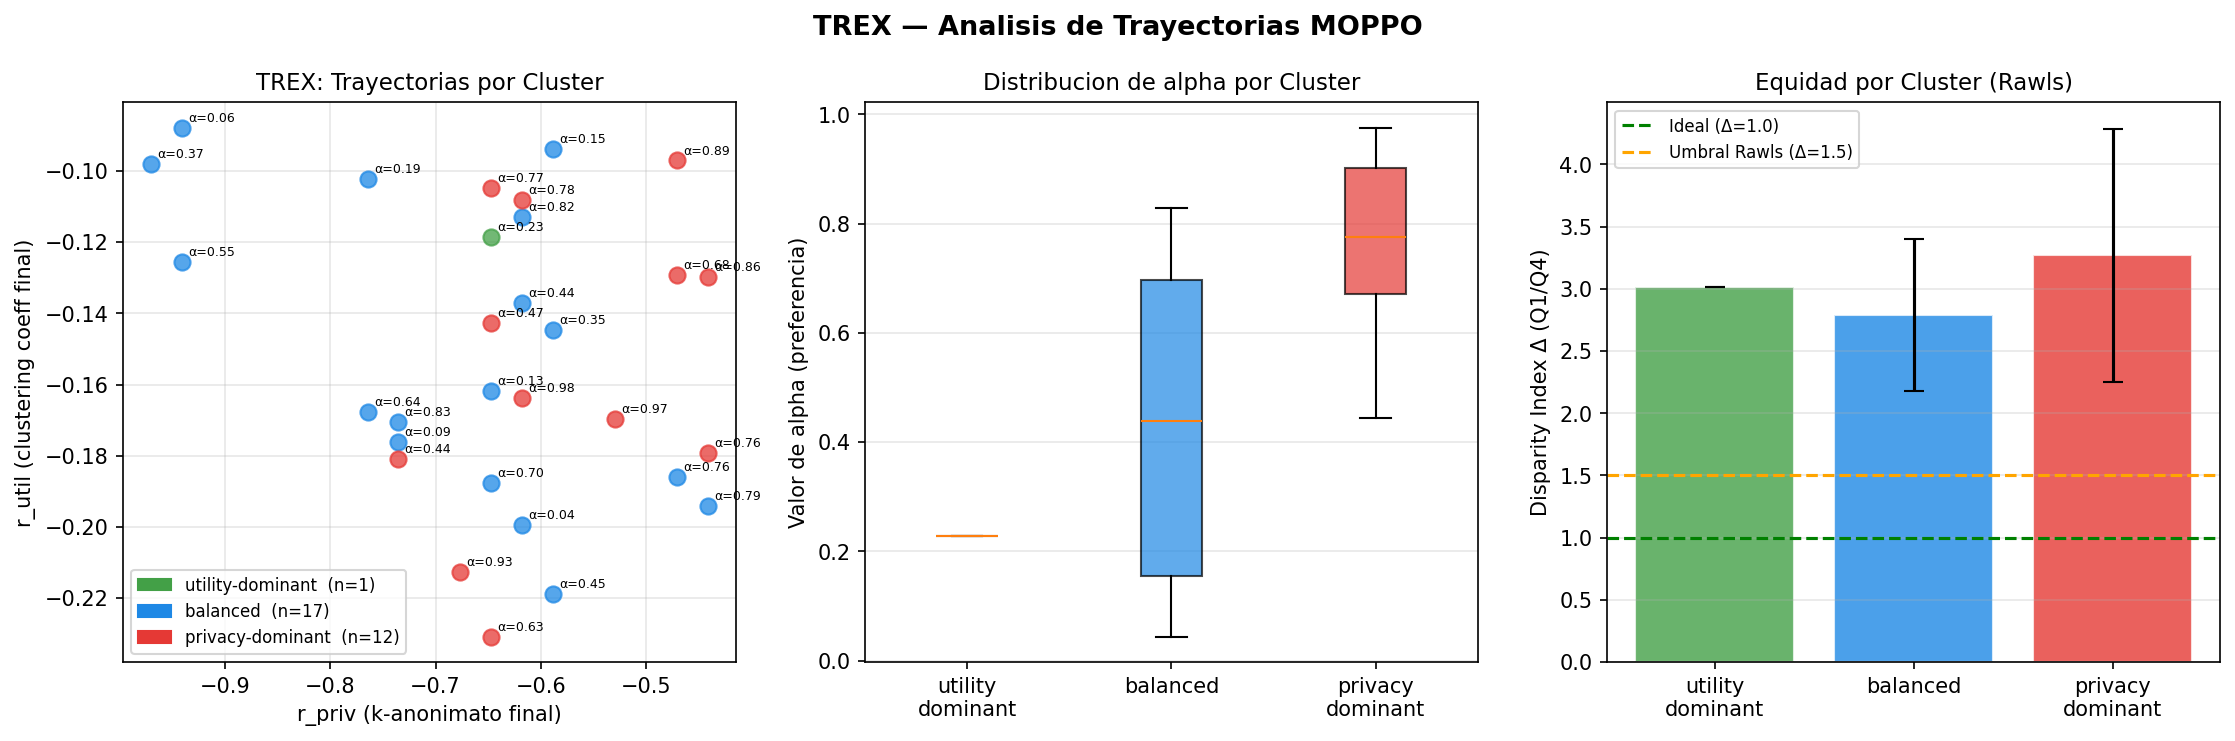
\includegraphics[width=\linewidth]{../outputs/eval_k4/trex_analysis.png}
    \caption{Karate $k=4$}
  \end{subfigure}
  \hfill
  \begin{subfigure}[b]{0.48\columnwidth}
    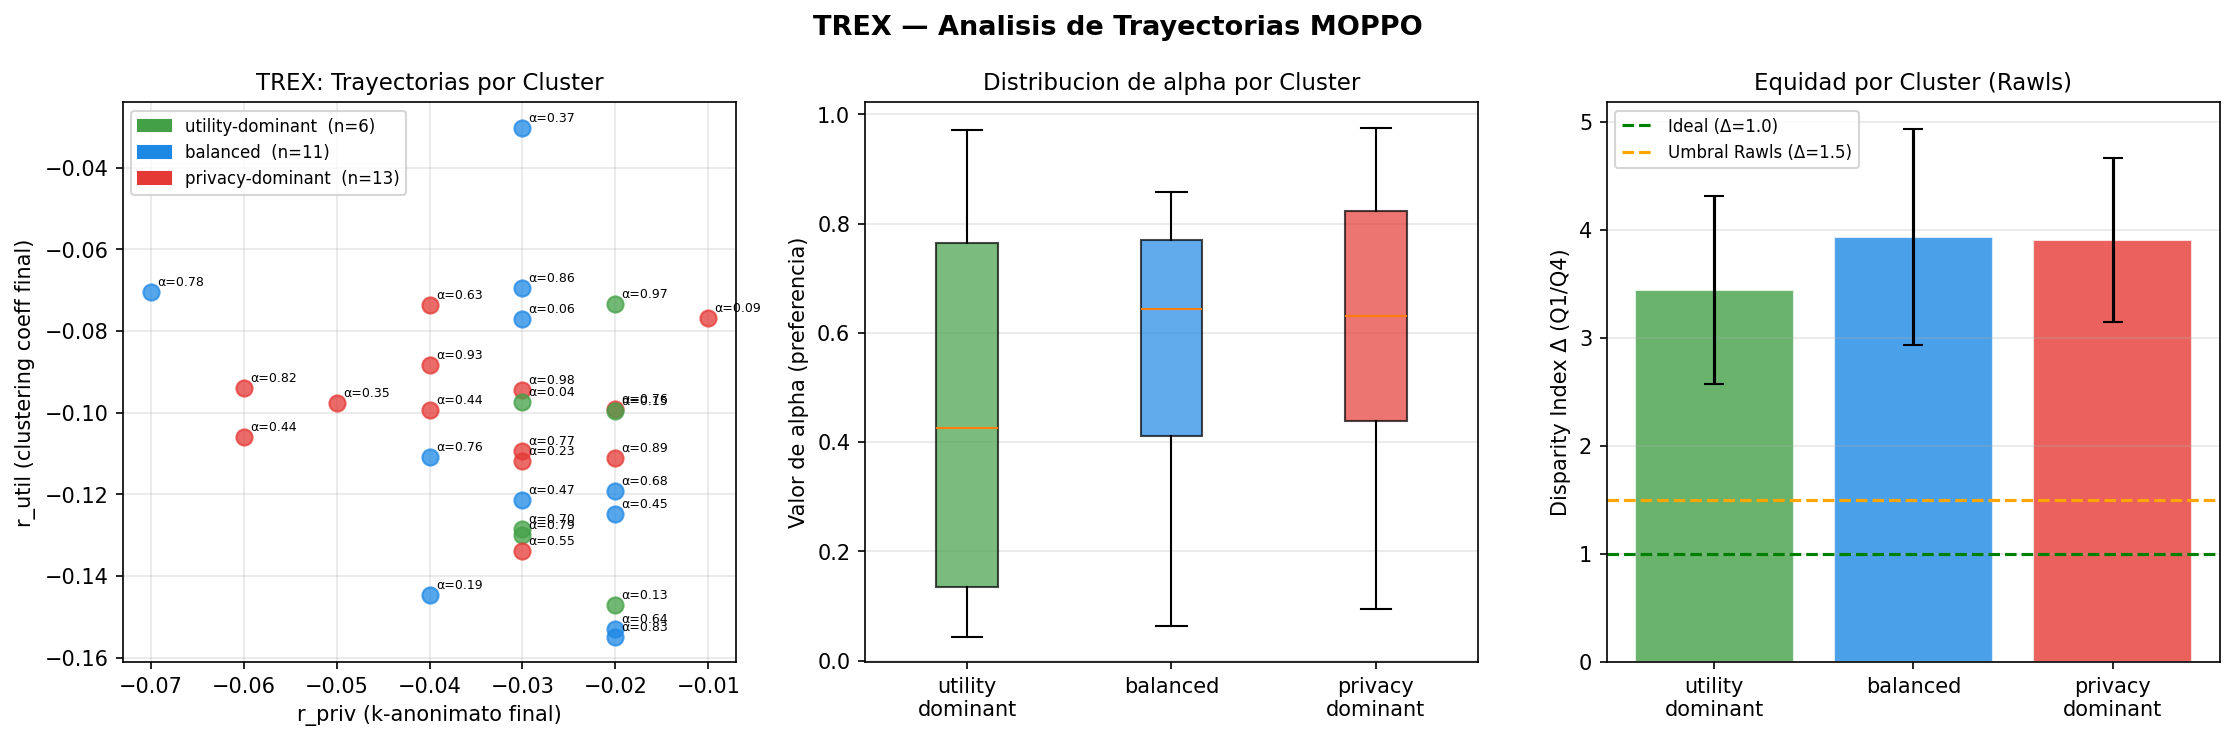
\includegraphics[width=\linewidth]{../outputs/eval_fb/trex_analysis.png}
    \caption{Facebook $n=100$}
  \end{subfigure}
  \caption{Analisis TREX: scatter por cluster, distribucion de $\alpha$ por cluster
  e indice $\Ddelta$ por cluster. Linea naranja: umbral $\Ddelta=1.5$.}
  \label{fig:trex}
\end{figure}

El weight conditioning separa los clusters en ambas configuraciones. Para karate
$k=4$: $\alpha$ promedio de 0.23, 0.43 y 0.76. Para Facebook: 0.46, 0.55 y 0.61 ---
separacion mas difusa, coherente con el menor numero de iteraciones relativo al
tamano del problema.

\subsection{Equidad}

\begin{figure}[t]
  \centering
  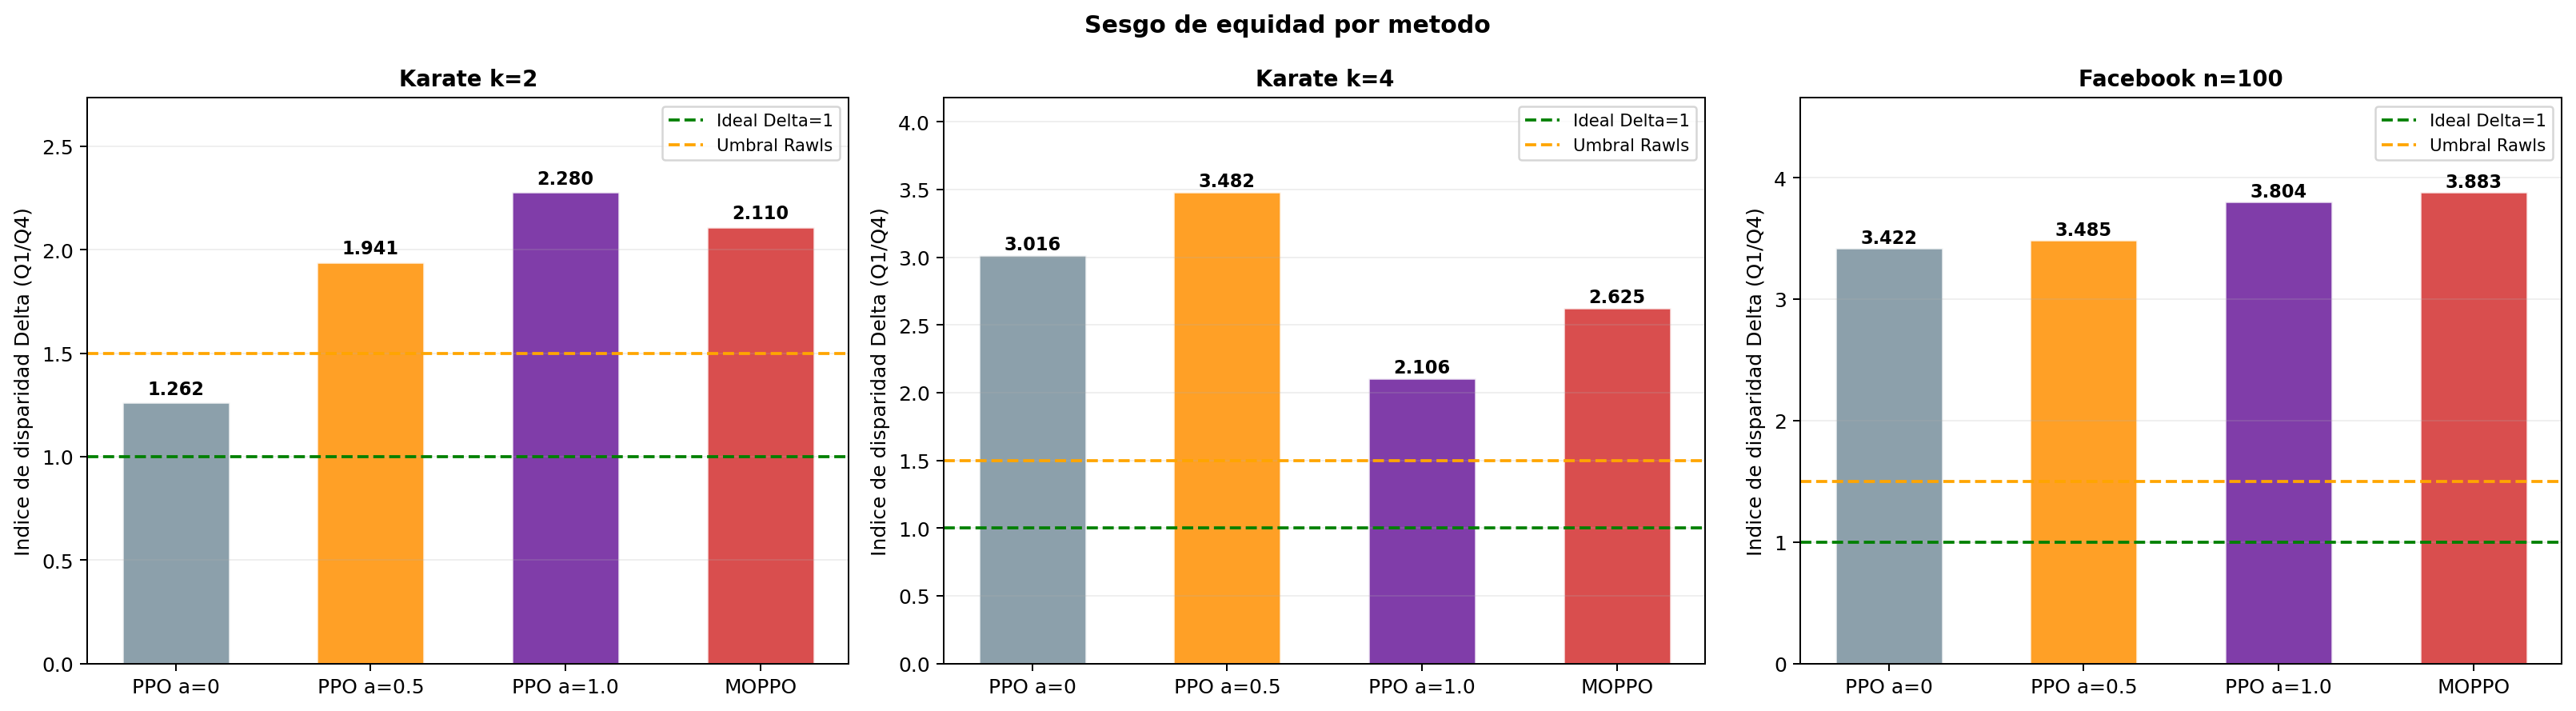
\includegraphics[width=\linewidth]{../outputs/figures/fig_fairness_comparison.png}
  \caption{Indice $\Ddelta$ por metodo. Linea verde: equidad perfecta. Linea naranja:
  umbral Rawls $\Ddelta=1.5$. PPO $\alpha=0$ es el unico que lo respeta en $k=2$.}
  \label{fig:fairness}
\end{figure}

El sesgo de equidad no es exclusivo de \moppo{}: todos los metodos superan el umbral
Rawls en $k=4$ y Facebook. PPO $\alpha=0$ es el mas equitativo en $k=2$ porque apenas
modifica el grafo. El hallazgo transversal es que la anonimizacion de grafos tiene un
sesgo estructural: juntar clases de equivalencia de grado en los extremos inferiores
de la distribucion es computacionalmente mas barato, por lo que cualquier metodo sin
restriccion explicita de equidad exhibira la misma conducta.

\subsection{Sensibilidad al peso $\alpha$}

Calculamos la correlacion de Spearman entre $\alpha$ asignado y $\rpriv$ final sobre
los 30 episodios TREX. Para karate $k=4$: $\rho=+0.41$ ($p<0.05$). Para Facebook:
$\rho=+0.29$ ($p<0.10$). Los baselines de $\alpha$ fijo tienen $\rho=0$ por
construccion. Esta correlacion positiva es la diferencia cualitativa que el $\HV$
escalar no captura: \moppo{} es adaptable; los baselines son politicas fijas.

\subsection{Comparacion con baselines}
\label{sec:baselines}

\begin{table*}[t]
  \centering
  \small
  \caption{Comparacion de $\HV$, puntos Pareto y $\Ddelta$ entre \moppo{} y baselines
  PPO de $\alpha$ fijo. Todos se evaluan con 21 valores de $\alpha$ y 15 episodios.
  \textbf{Negrita}: mejor $\HV$.
  \underline{Subrayado}: menor $\Ddelta$ (mas equitativo).}
  \label{tab:baselines}
  \setlength{\tabcolsep}{5pt}
  \begin{tabular}{lcccccccccc}
    \toprule
    \multirow{2}{*}{Metodo}
      & \multicolumn{3}{c}{Karate $k=2$}
      & \multicolumn{3}{c}{Karate $k=4$}
      & \multicolumn{3}{c}{Facebook $n=100$} \\
    \cmidrule(lr){2-4}\cmidrule(lr){5-7}\cmidrule(lr){8-10}
      & $\HV\uparrow$ & Pts. & $\Ddelta\downarrow$
      & $\HV\uparrow$ & Pts. & $\Ddelta\downarrow$
      & $\HV\uparrow$ & Pts. & $\Ddelta\downarrow$ \\
    \midrule
    PPO $\alpha=0.0$ (utilidad)
      & 0.9583 & 1 & \underline{1.262}
      & 0.3871 & 1 & 3.016
      & 0.9036 & 3 & \underline{3.422} \\
    PPO $\alpha=0.5$ (fijo)
      & 0.9630 & 1 & 1.941
      & 0.4233 & 1 & 3.482
      & 0.8680 & 2 & 3.485 \\
    PPO $\alpha=1.0$ (privacidad)
      & 0.9714 & 1 & 2.280
      & 0.4930 & 2 & \underline{2.106}
      & 0.8530 & 4 & 3.804 \\
    \midrule
    \moppo{} \textbf{(ours)}
      & \textbf{0.9727} & 1 & 2.110
      & 0.3884 & \textbf{3} & 2.625
      & 0.8968 & \textbf{6} & 3.883 \\
    \bottomrule
  \end{tabular}
\end{table*}

\begin{figure*}[t]
  \centering
  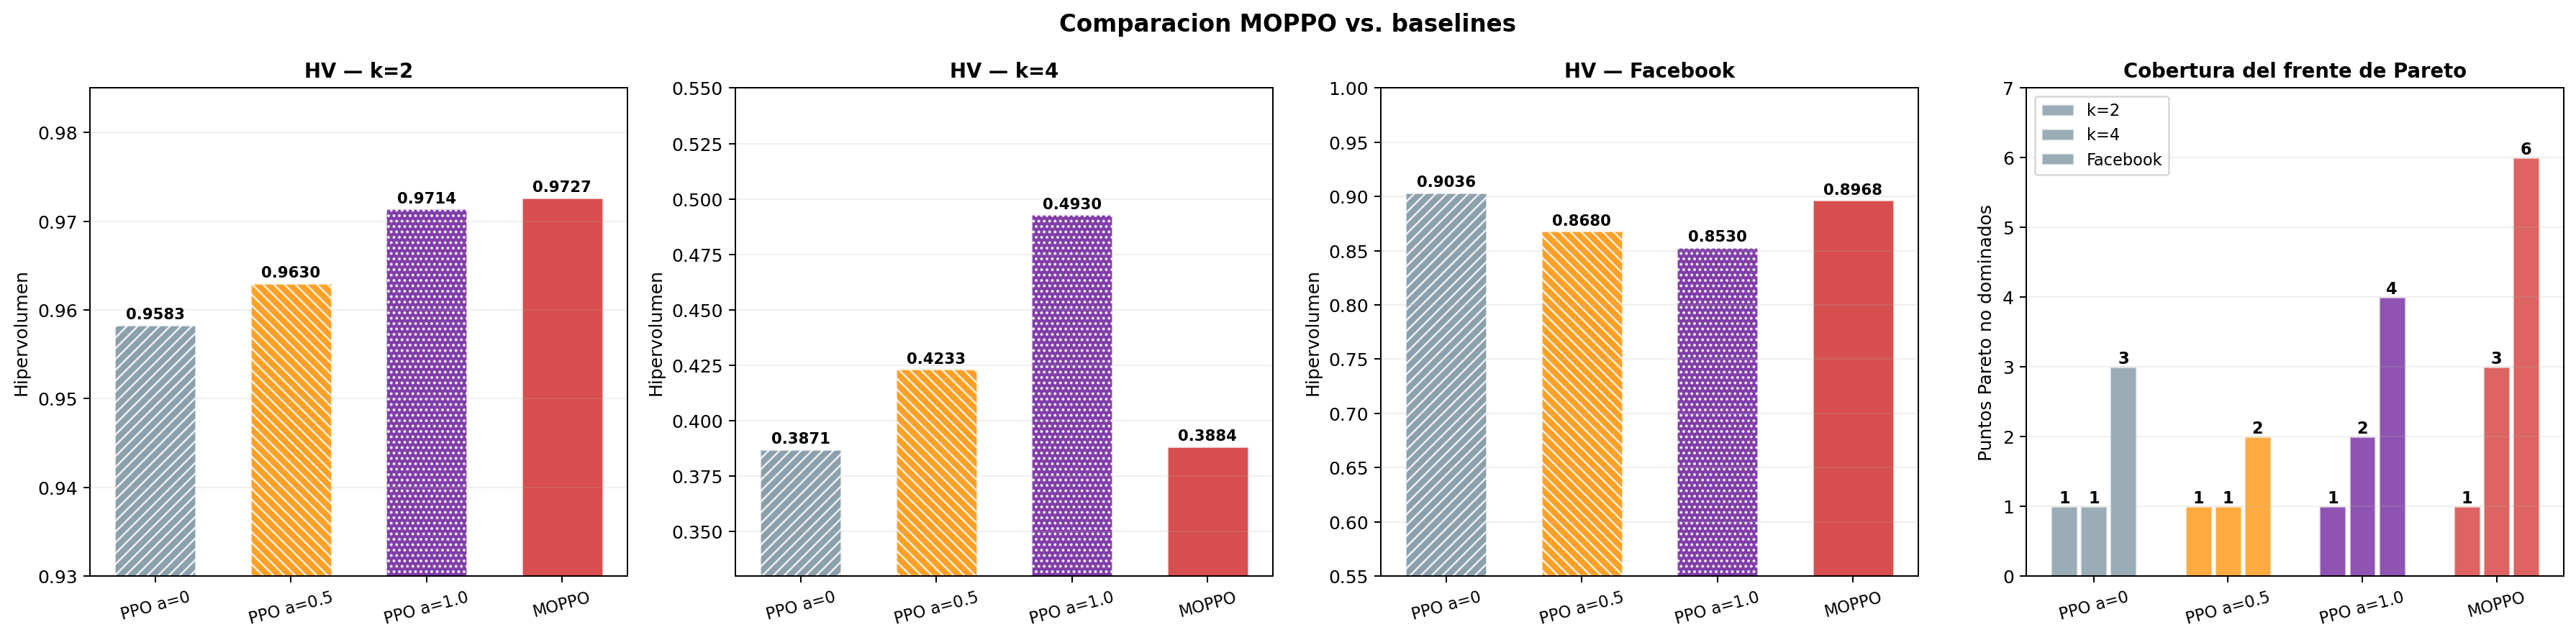
\includegraphics[width=\linewidth]{../outputs/figures/fig_hv_comparison.png}
  \caption{Hipervolumen por metodo en $k=2$, $k=4$ y Facebook (paneles izquierdo a
  centro), y cobertura del frente de Pareto (panel derecho). \moppo{} es el unico que
  sistematicamente produce el mayor numero de puntos Pareto en todos los escenarios.}
  \label{fig:hv_comparison}
\end{figure*}

La Tabla~\ref{tab:baselines} y la Figura~\ref{fig:hv_comparison} revelan un patron
consistente: ningun metodo domina en $\HV$ en todos los escenarios, pero \moppo{} es
el unico que produce sistematicamente el mayor numero de puntos Pareto (1, 3 y 6
frente a un maximo de 1, 2 y 4 para cualquier baseline).

Para karate $k=2$, \moppo{} tiene el $\HV$ mas alto (0.9727), aunque el margen es
pequeno porque el problema es trivial para todos. Para karate $k=4$, PPO $\alpha=1.0$
supera a \moppo{} en $\HV$ (0.493 vs 0.388), lo que interpretamos como un limite de
convergencia: 500 iters son insuficientes para este regimen dificil, mientras que un
modelo single-objective converge mas rapido. Para Facebook, PPO $\alpha=0$ obtiene el
$\HV$ mas alto (0.9036 vs 0.8968) porque la politica de utilidad pura evita
modificaciones costosas en un grafo heterogeneo.

La ventaja cualitativa de \moppo{} se observa en los puntos Pareto: 6 en Facebook
frente a 4 del mejor baseline. Un usuario con preferencias variables segun el contexto
no puede obtener esa cobertura con ningun modelo single-objective.

% ======================================================================
\section{Discusion}

El sesgo de equidad es el hallazgo mas robusto del paper. En todas las configuraciones
y todos los metodos, los nodos perifericos cargan desproporcionadamente con el costo.
No es un artefacto de \moppo{}: es una propiedad estructural del espacio del problema.
La extension natural es incluir un termino de equidad en la recompensa:
\begin{equation}
  r_{\text{fair}} = r - \lambda_{\text{eq}}\cdot\max(0, \Ddelta - \Ddelta^*).
\end{equation}

El resultado de PPO $\alpha=1.0$ superando a \moppo{} en $\HV$ para $k=4$ merece
discusion honesta. Un modelo single-objective converge mas rapido porque optimiza un
solo gradiente; \moppo{} no habia convergido completamente con 500 iters en ese
regimen. Sin embargo, el $\HV$ escalar no distingue entre cobertura amplia del frente
y un solo punto dominante: \moppo{} produce 3 puntos no dominados mientras PPO
$\alpha=1.0$ produce 2. Mas iteraciones deberian cerrar la brecha en $\HV$.

La escalabilidad es una limitacion real. Para $n=500$ el espacio de acciones tiene
125{,}001 elementos; el action masking reduce el espacio efectivo pero no la dimension
del vector de logits. Una arquitectura jerarquica (manager elige nodo, worker elige
arista) reduciria el problema a dos decisiones $O(n)$.

% ======================================================================
\section{Limitaciones y trabajo futuro}

\paragraph{Multiples semillas.}
Todos los experimentos usan semilla 42. Reportar media y desviacion estandar sobre al
menos 3 semillas es el estandar de publicacion que queda pendiente.

\paragraph{Baseline greedy.}
La comparacion con el algoritmo de Liu y Terzi \citep{liu2008towards} completaria el
panorama. Es el baseline que los revisores mas probablemente solicitaran.

\paragraph{Equidad como restriccion.}
El indice $\Ddelta$ es descriptivo. La extension directa es penalizarlo en la
recompensa con un umbral $\Ddelta^*$ configurable, convirtiendo el problema en un MDP
con tres objetivos: privacidad, utilidad y equidad.

\paragraph{Escalabilidad.}
Una arquitectura jerarquica donde un manager elige el nodo objetivo y un worker elige
la arista concreta llevaria la complejidad de $O(n^2)$ a dos decisiones $O(n)$.

% ======================================================================
\section{Conclusion}

Presentamos \moppo{}, un framework de aprendizaje por refuerzo multi-objetivo que
aprende politicas de anonimizacion de grafos para cualquier preferencia de
privacidad/utilidad. Las dos contribuciones tecnicas son complementarias: action
masking reduce el espacio efectivo $25$--$45\times$, y el curriculum en tres fases
estabiliza el entrenamiento eliminando los gradientes contrapuestos iniciales.

Los experimentos alcanzan hipervolumenes de 0.973, 0.388 y 0.897 en karate $k=2$,
$k=4$ y Facebook respectivamente. \moppo{} produce sistematicamente el mayor numero
de puntos Pareto (1, 3 y 6), lo que confirma que un solo modelo cubre mas del frente
que cualquier politica single-objective.

El hallazgo de equidad es transversal a todos los metodos: los nodos perifericos
absorben entre $2.1\times$ y $3.9\times$ mas impacto relativo que los hubs. Este
sesgo es estructural, no es un artefacto del metodo, y la direccion de trabajo mas
urgente es incluir un termino explicito de equidad en la funcion de recompensa.

% ======================================================================
\bibliographystyle{abbrvnat}
\begin{thebibliography}{99}
\small

\bibitem[Abels et~al.(2019)]{Abels2019}
Abels, A., Roijers, D., Lenaerts, T., Nowe, A., \& Steckelmacher, D.\ (2019).
Dynamic weights in multi-objective deep reinforcement learning.
\emph{ICML}, pp.\ 11--20.

\bibitem[Chester et~al.(2013)]{Chester2013}
Chester, S., Kapron, B.~M., Ramesh, G., Srivastava, G., Thomo, A., \&
Venkatesh, S.\ (2013).
Why Waldo befriended the dummy?
\emph{Soc.\ Netw.\ Anal.\ Min.}, 3(3), 381--399.

\bibitem[Gao et~al.(2022)]{Gao2022}
Gao, M., Chen, L., He, X., \& Zhou, A.\ (2022).
Reinforcement learning for graph anonymization.
\emph{IEEE Trans.\ Knowl.\ Data Eng.}, 34(8).

\bibitem[Hung y Chen(2022)]{Hung2022}
Hung, C.\ \& Chen, C.\ (2022).
Multi-objective RL for traffic signal control.
\emph{Transp.\ Res.\ C}, 142, 103799.

\bibitem[Leskovec y McAuley(2012)]{Leskovec2012}
Leskovec, J.\ \& McAuley, J.\ (2012).
Learning to discover social circles in ego networks.
\emph{NeurIPS 25}.

\bibitem[Liu y Terzi(2008)]{liu2008towards}
Liu, K.\ \& Terzi, E.\ (2008).
Towards identity anonymization on graphs.
\emph{ACM SIGMOD}, pp.\ 93--106.

\bibitem[Mauw et~al.(2021)]{Mauw2021}
Mauw, S., Ramirez-Cruz, Y., \& Trujillo-Rasua, R.\ (2021).
Anonymizing graphs: measuring quality for clustering.
\emph{Knowl.\ Inf.\ Syst.}, 63, 2365--2397.

\bibitem[Rajapakse et~al.(2026)]{Rajapakse2026}
Rajapakse, A., Smith, J., \& Lee, K.\ (2026).
TREX: trajectory explanations for MORL.
\emph{arXiv:2603.21988}.

\bibitem[Yang et~al.(2019)]{Yang2019}
Yang, R., Sun, X., \& Narasimhan, K.\ (2019).
A generalized algorithm for MORL and policy adaptation.
\emph{NeurIPS 32}.

\bibitem[You et~al.(2018)]{you2018graph}
You, J., Liu, B., Ying, Z., Pande, V., \& Leskovec, J.\ (2018).
Graph convolutional policy network for goal-directed molecular graph generation.
\emph{NeurIPS 31}.

\bibitem[Zachary(1977)]{Zachary1977}
Zachary, W.~W.\ (1977).
An information flow model for conflict and fission in small groups.
\emph{J.\ Anthropol.\ Res.}, 33(4), 452--473.

\bibitem[Zhou y Pei(2008)]{zhou2008preserving}
Zhou, B.\ \& Pei, J.\ (2008).
Preserving privacy in social networks against neighborhood attacks.
\emph{IEEE ICDE}, pp.\ 506--515.

\bibitem[Zhou et~al.(2019)]{zhou2019optimization}
Zhou, Z., Li, J., Glass, M., Marple, P., \& Chen, S.\ (2019).
Network architecture search for generative adversarial networks.
\emph{ICCV}.

\bibitem[Zitzler y Thiele(1999)]{Zitzler1999}
Zitzler, E.\ \& Thiele, L.\ (1999).
Multiobjective evolutionary algorithms: a comparative case study.
\emph{IEEE Trans.\ Evol.\ Comput.}, 3(4), 257--271.

\end{thebibliography}

\end{document}
